%
\section{Software specification}
\label{sec:sw-specs}
Next, the \gls{sw} responsible for system operation is specified for all
subsystems --- \texttt{\acrfull{mdo-rc}}, \texttt{\acrfull{mdo-rs}}, and
\texttt{\acrfull{mdo-l}}.
All these subsystems are event-driven (asynchronous), and they can be more easily
specified using state-machine diagrams, previously illustrated in the
\emph{analysis phase} (Section~\ref{sec:softw-arch}). Also in the \emph{analysis
phase}, the use case diagrams helped to identify the main features required for
the system and the respective sequence diagrams helped to clarify the
intervening objects and the interaction among them.

In this section, the analysis phase information is used to derive the static
architecture of the system --- classes diagram --- and to specify algorithms for
its implementation through flowcharts, keeping in mind that the several
subsystems operate multiple tasks concurrently, thus requiring the tasks'
specification and its priorities. The data frame formats are specified for
communication between the different modules. The \acrfull{erd} are depicted to
design the required databases and the \gls{ui} mock-ups are recalled. The test
cases for each subsystem are listed, defining its operation and the expected
result. The \gls{cots} \gls{sw} and the third-party libraries are identified
and a mapping between class topics and the foreseeable implementation is
presented for clarification. Finally, the \gls{sw} tools are listed.

\subsection{Software architecture}
\label{sec:softw-arch-1}
The system's \gls{sw} architecture was devised using \emph{\gls{uml} component
  diagrams} for \texttt{Remote Client} (Fig.~\ref{fig:component-diag-rc}), \texttt{Remote Server} (Fig.~\ref{fig:component-diag-rs}), and
\texttt{Local System} (Fig.~\ref{fig:component-diag-local}). Each component
diagram illustrates all \gls{sw} components for the system in analysis and the
interaction between them, and its
interfaces with external subsystems.

\subsubsection{Remote Client}
\label{sec:remote-client-arch}
Fig.~\ref{fig:component-diag-rc} depicts the \texttt{Remote Client} \gls{sw} architecture, encapsulated in the package
\texttt{MDO-RC: AppManager}, and is comprised of the following artifacts:
\begin{item-c}
\item
  \emph{\texttt{User Interface} package}: contains the \texttt{\gls{ui}} and
  \texttt{\gls{ui} Engine}. It is responsible for providing user feedback and
  capturing \gls{ui} events which drive the \texttt{Remote Client}'s logic.
\item
  \emph{\texttt{Comm Manager} package}: manages incoming and outgoing
  connections to the \texttt{Remote Server} (package \texttt{MDO-RS: App Manager}), periodically checking the
  connection status by pinging the \texttt{Remote Server}. All connections
  consist of \gls{tcp-ip} sockets.
\item
  \emph{\texttt{DB Manager} package}: manages the queries and the associated
  responses by building or parsing them, respectively.
\item 
  \emph{\texttt{Remote Controller} package}: contains the \texttt{Cmd Parser},
  which parses the command responses received from the \texttt{Remote Server}
  when the \texttt{Admin} is performing remote control of the \texttt{Local
    System}.
\item
  \emph{\texttt{RC Rx Parser} component}: high-level parser which filters
  between \texttt{db responses} and \texttt{cmd responses} for appropriate
  dispatching.
\item
  \emph{\texttt{\gls{tcp-ip} Tx} socket}: outgoing connection node, through
  which \texttt{tx frames} are sent to the \texttt{Remote Server}.
\item 
  \emph{\texttt{\gls{tcp-ip} Rx} socket}:  incoming connection node, through
  which \texttt{rx frames} are received from the \texttt{Remote
    Server}.
\end{item-c}

\begin{figure}[htb!]
\centering
    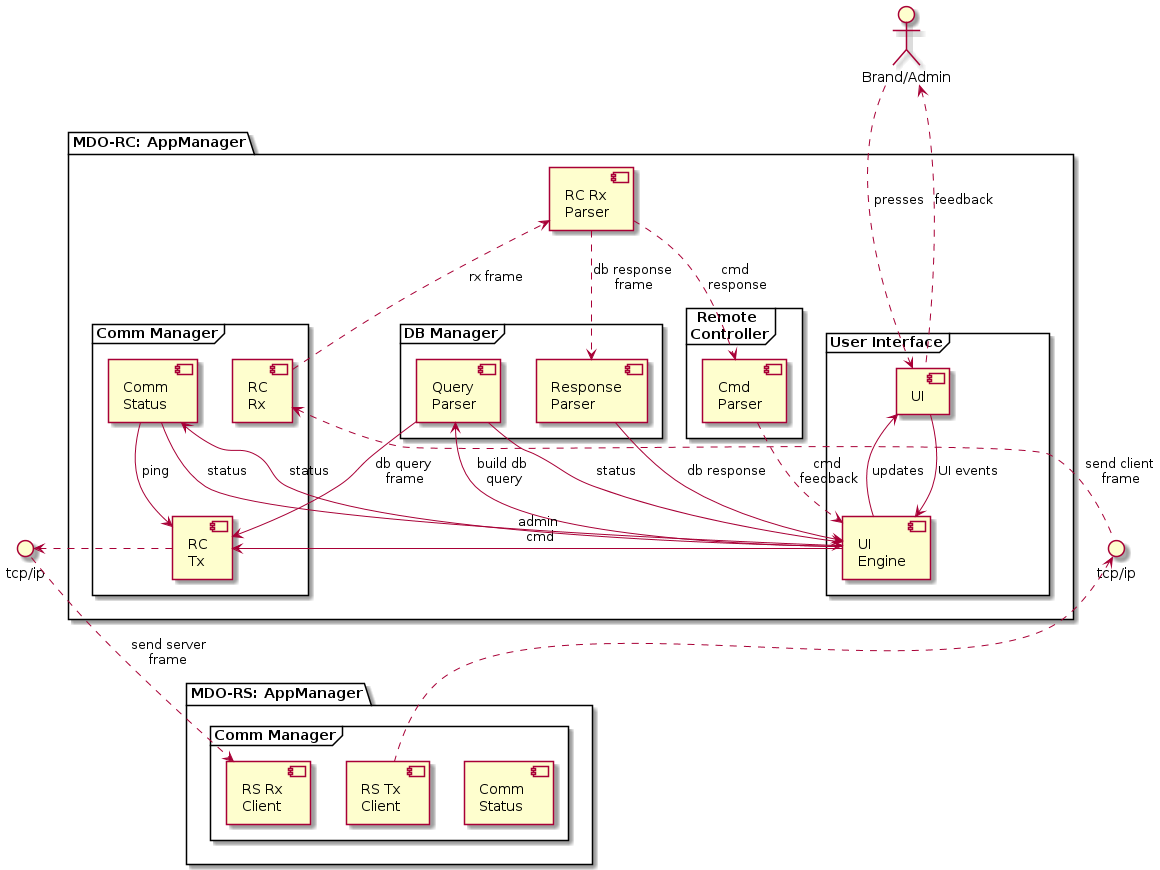
\includegraphics[width=0.9\columnwidth]{./img/component-diag-rc.png}
  \caption{\gls{sw} architecture: component diagram --- \texttt{Remote Client}}%
\label{fig:component-diag-rc}
\end{figure}

\subsubsection{Remote Server}
\label{sec:remote-server-arch}
Fig.~\ref{fig:component-diag-rs} depicts the \texttt{Remote Server} \gls{sw} architecture, encapsulated in the package
\emph{\texttt{MDO-RS: AppManager}}. It interacts with the \texttt{Remote Client}
(package \texttt{MDO-RC: AppManager}), with the \texttt{Local System} (package
\texttt{MDO-L: AppManager}), and with the \texttt{\gls{db} server}
(\texttt{MDO-RS: DB Server}). The database management is done using
client-server architecture, with \texttt{MDO-RS: AppManager} containing the
\gls{db} client and \texttt{MDO-RS: DB Server} the server.
%
\begin{figure}[htb!]
\centering
    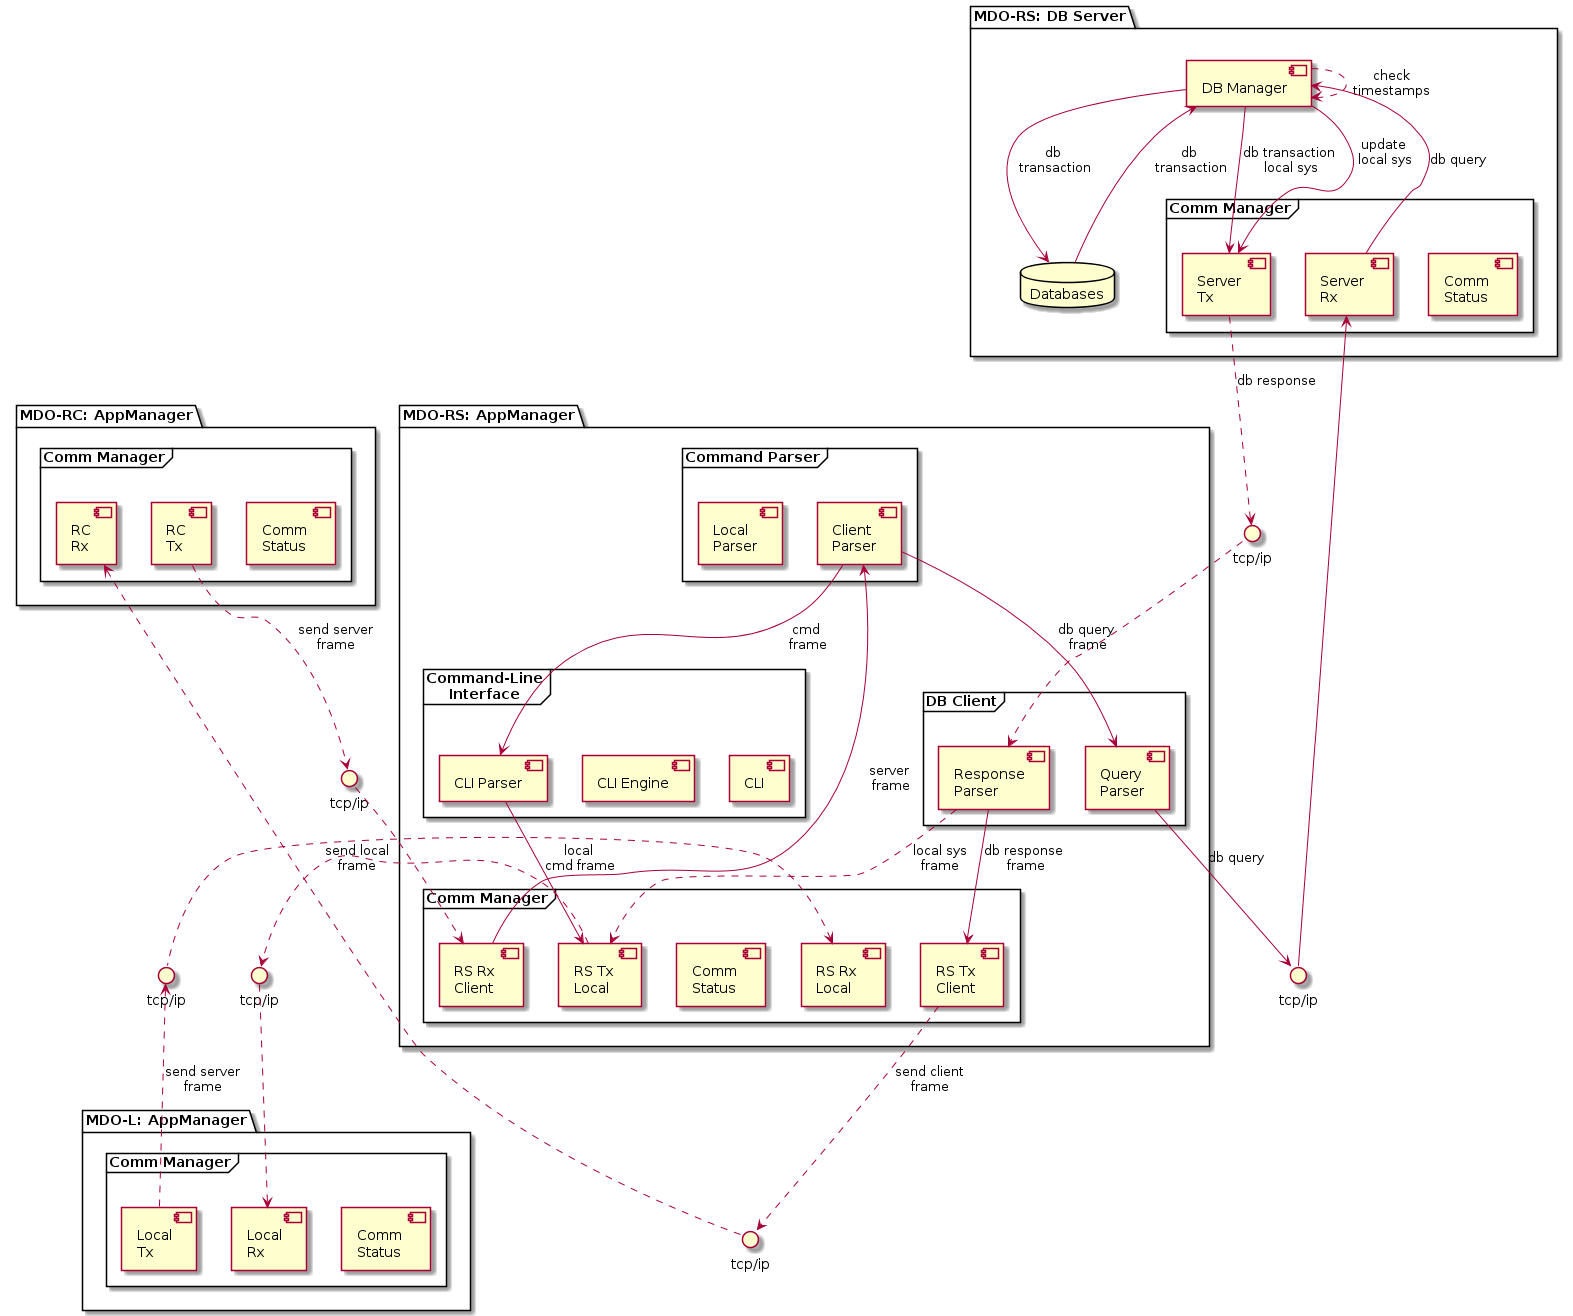
\includegraphics[width=1.0\columnwidth]{./img/component-diag-rs.png}
  \caption{\gls{sw} architecture: component diagram --- \texttt{Remote Server}}%
\label{fig:component-diag-rs}
\end{figure}

The \emph{\texttt{MDO-RS: AppManager}} package is comprised of the following artifacts:
\begin{item-c}
\item
  \emph{\texttt{Command--Line Interface} package}: contains the
  \texttt{\gls{cli}}, the
  \texttt{\gls{cli} Engine}, and the \texttt{\gls{cli} Parser}. It provides the
  server external interface for clients to perform requests,
  capturing the events which drive the \texttt{Remote Server}'s logic.
\item
  \emph{\texttt{Comm Manager} package}: manages incoming and outgoing
  connections to the \texttt{Remote Client} (package \texttt{MDO-RC: App
    Manager}),  and each \texttt{Local System} (package \texttt{MDO-L:
    AppManager}) it needs to interact. It periodically checks all
  connections statuses. All connections
  consist of \gls{tcp-ip} sockets.
\item
  \emph{\texttt{DB Client} package}: manages the queries and the associated
  responses by building or parsing them, respectively. It performs the requests
  for \texttt{\gls{db} server} with the solicited queries.
\item 
  \emph{\texttt{Command Parser} package}: contains the \texttt{Client Parser},
  and the \texttt{Local Parser} to parse and handle frames received from the
  \texttt{Remote Client} or \texttt{Local System}, respectively, forwarding it
  for appropriate dispatching.
\item
  \emph{\gls{tcp-ip} sockets}: incoming/outgoing connection nodes, through which
  incoming or outgoing traffic flows for the \texttt{Remote Client}, the
  \texttt{Local System} and the \texttt{DB Server}.
\end{item-c}

\vspace{1em}
The \emph{\texttt{MDO-RS: DB Server}} package is comprised of the following artifacts:
\begin{item-c}
\item
  \emph{\texttt{Comm Manager} package}: manages incoming and outgoing
  connections to the \texttt{DB Client} (in package \texttt{MDO-RS: App
    Manager}). It periodically checks all
  connections statuses. All connections
  consist of \gls{tcp-ip} sockets.
\item
  \emph{\texttt{DB Manager} package}: handles the received queries, issuing
  transactions for the databases and returns its response. It is also
  responsible for periodically checking timestamps, and when there is a match,
  update the local system with the relevant information.
\item
  \emph{Databases}: contains the actual data stored.
\end{item-c}
%
\subsubsection{Local System}
\label{sec:local-system-arch}
Fig.~\ref{fig:component-diag-local} depicts the \texttt{Local System} \gls{sw} architecture, encapsulated in the package
\emph{\texttt{MDO-L: AppManager}}.
%
\begin{figure}[htb!]
\centering
    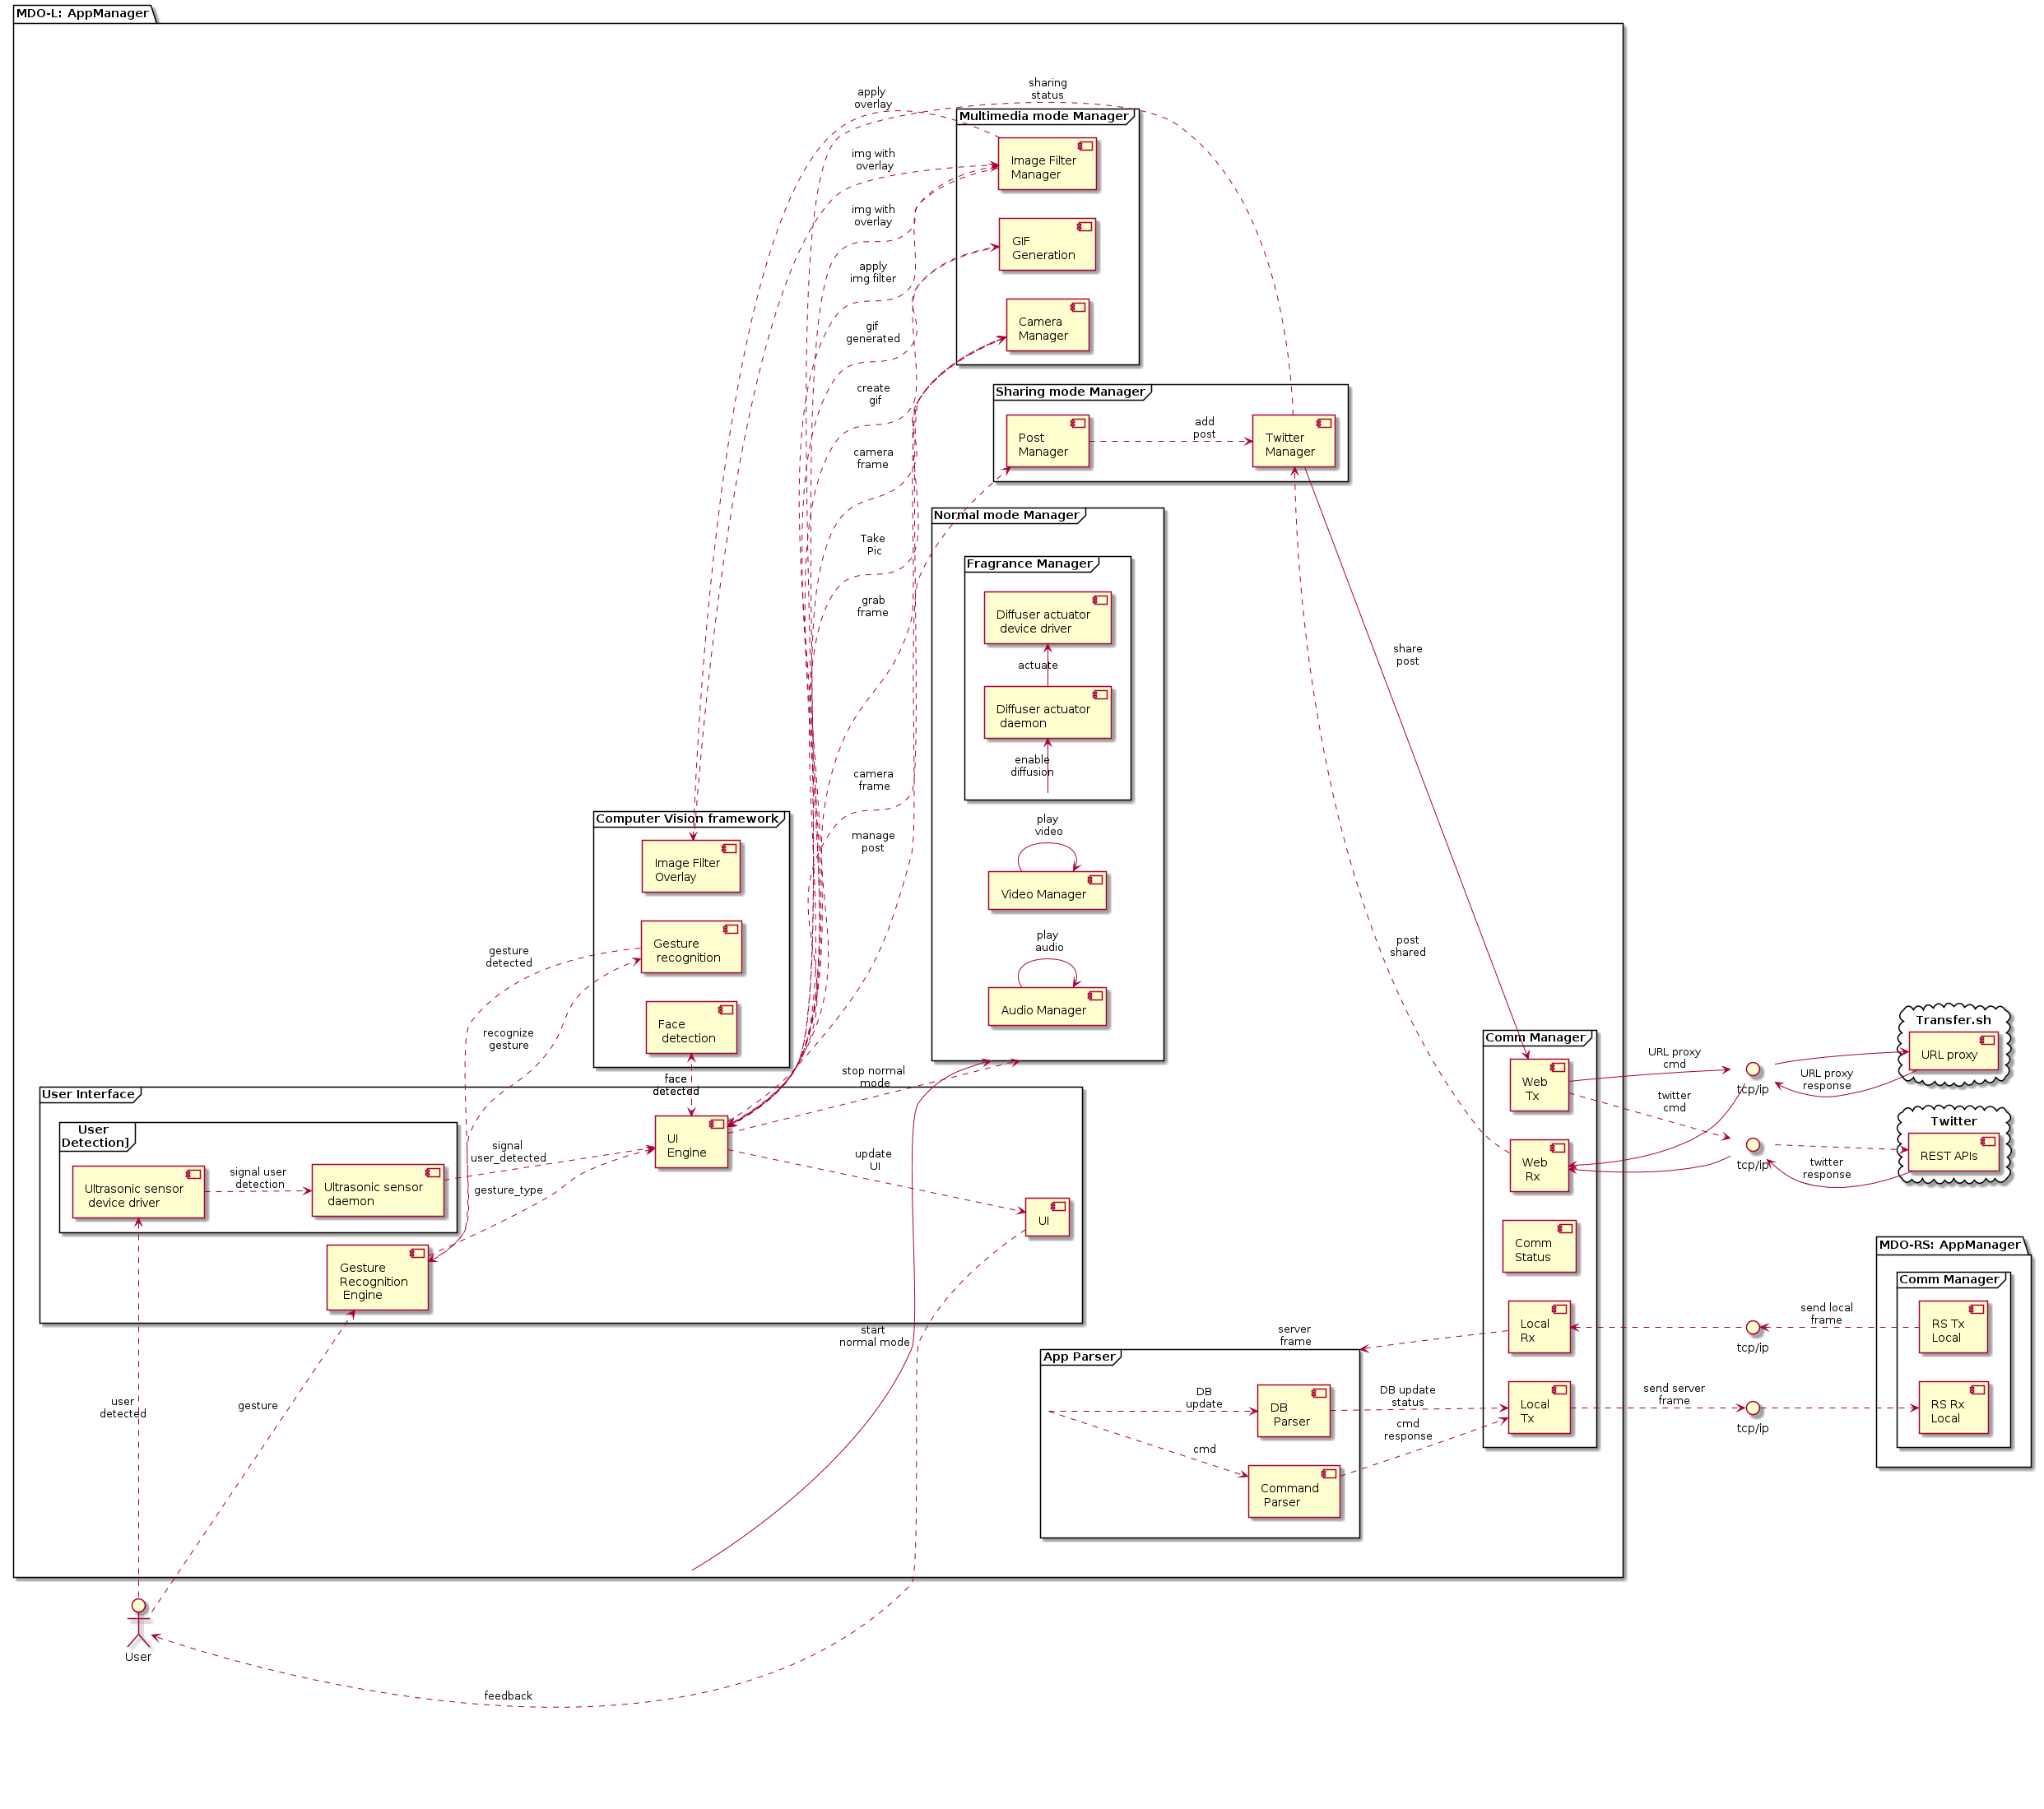
\includegraphics[width=1.03\columnwidth]{./img/component-diag-local.png}
  \caption{\gls{sw} architecture: component diagram --- \texttt{Local system}}%
\label{fig:component-diag-local}
\end{figure}

It interacts with:
\begin{item-c}
\item 
\emph{\texttt{Remote Server}} (package \texttt{MDO-RS: AppManager}): to retrieve updates on its operation or
\texttt{Admin} commands
\item
  \emph{\texttt{Twitter}} (via its \texttt{\gls{rest} \glspl{api}}): to share
  posts on it
\item
  \texttt{transfer.sh} --- an \gls{url} proxy server: to ease file transfer
  between the \texttt{Remote Server} and the \texttt{Local System}.
\end{item-c}

\vspace{1em}
The \emph{\texttt{MDO-RS: AppManager}} package is comprised of the following artifacts:
\begin{item-c}
\item
  \emph{\texttt{User Interface} package}: contains the \texttt{\gls{ui}}, the
  \texttt{\gls{ui} Engine}, the \texttt{Gesture Recognition Engine}, and the
  \texttt{User Detection package}. The \texttt{\gls{ui}} provides user feedback
  and \texttt{UI Engine}
  captures the events that drive the \texttt{Local System}'s logic. When a user
  approaches the \texttt{Local System}, the \texttt{Ultrasonic sensor device
    driver} captures this event and passes it to the user space where the
  \texttt{Ultrasonic sensor daemon} logs it, which, in turn, signals this event
  to the \texttt{UI Engine}. When the \texttt{User} performs gestures, the
  \texttt{Gesture Recognition Engine} requires a service to the \texttt{Gesture
    recognition} component (\texttt{Computer Vision Framework}) to recognize the
  gesture. Also, when the \texttt{User} is detected, the \texttt{UI Engine}
  requests the \texttt{Normal mode manager} to stop running, and requests
  \texttt{Face detection} to track people's faces in the camera.
\item
  \emph{\texttt{Comm Manager} package}: manages incoming and outgoing
  connections to the \texttt{Remote Server} (package \texttt{MDO-RS: App
    Manager}),  and the internet for each web service it needs to interact
  (\texttt{Twitter} and \texttt{transfer.sh}).
  It periodically checks all connections statuses. All connections
  consist of \gls{tcp-ip} sockets.
\item
  \emph{\texttt{Computer Vision framework} package}: manages the computer vision
  related tasks, namely, gesture recognition, face detection, and image filter
  overlay.
\item 
  \emph{\texttt{Multimedia Mode Manager} package}: manages the multimedia mode
  related tasks, namely, image filtering, \gls{gif} generation, and camera
  management.
\item 
  \emph{\texttt{Sharing Mode Manager} package}: manages the sharing mode
  related tasks, namely, post management, and social media management, in this
  case, \texttt{Twitter}.
\item 
  \emph{\texttt{Normal Mode Manager} package}: manages the normal mode
  related tasks, namely, fragrance diffusion, video and audio outputs. The
  fragrance diffusion is requested to the device driver using a daemon to bridge
  user-space and kernel-space.
\item 
  \emph{\texttt{App Parser} package}: manages the parsing for database queries
  and requested commands.
\item
  \emph{\gls{tcp-ip} sockets}: incoming/outgoing connection nodes, through which
  incoming or outgoing traffic flows for the \texttt{Remote Server}, and the web
  services for \texttt{Twitter} and the \texttt{\gls{url} proxy server}.
\end{item-c}
%
%

\subsection{Static architecture --- Class diagrams}
\label{sec:stat-arch-class}
In this section the static architecture is derived from the \gls{sw}
architecture, i.e., the class diagrams are outlined, using the component
diagrams as a starting point, for each subsystem.

\subsubsection{Remote Client}
\label{sec:remote-client-class}

\subsubsection{Remote Server}
\label{sec:remote-server-class}

\subsubsection{Local System}
\label{sec:local-system-class}



\section{Software interfaces definition}
\label{sec:sw-interf-def}
%- Define the APIs in detail:
%  - header files with:
%    - functions prototypes
%    - data structure declarations
%    - class declarations
%
% From the state machine diagram (Fig.~\ref{fig:state-mach}) the softwares modules
% and data structures can be infered. The data structure is \texttt{keycode\_fifo},
% a circular buffer to manage the keycodes produced and consumed. The modules are
% \texttt{i2c}, \texttt{ir} and \texttt{fifo} for determing the key pressed,
% transmitting the keycode and managing the \gls{fifo} buffer. Enumerations are
% added for keycodes and errors listing.
% 
% An example of the \gls{api} can be seen in Listing~\ref{lst:api}, using builtin documentation.
% %
% \lstinputlisting[language=c, firstline=1,caption={\gls{api} example with
%   builtin documentation},label=lst:api,
% style=customc]{./listing/api.h}%

\section{Start-up/shutdown process specification}
\label{sec:startup-shutdown}
%As highlighted in Fig.~\ref{fig:state-mach}, the process starts with battery
%power being supplied to the system, going into sleep mode and waiting for
%events, minimizing power consumption. However, there is still residual power
%being drawn. This could be overcome by placing a power button for the remote
%itself, but with the inconvenience of MCU reset and the initial delays
%associated. The shutdown results from batteries disconnection.\

\section{Error handling specification}
\label{sec:error-handling-specification}
%Every system is prone to glitches, bugs and errors, thus, requiring it to be
%handled. Errors should be handled gracefully by creating error handling
%routines, which try to circumvent them and provide feedback.
%
%For extreme cases, where this is not possible, the watchdog timer should be
%enabled to help the system recover from crashes. However, this is a last resort,
%as constant reboots --- sign of a bad design --- are inadmissible and will
%frustrate the user.
%
%The error handling routines can be built into the design by considering return
%codes and asserts from function calls, e.g., \texttt{int i2c\_read(char *byte)},
%where \texttt{0} signals success and otherwise an error was encountered. Thus,
%good design eases error-handling specification and should be an aspect to keep
%in mind in this phase.
%%

\section{Test cases}
\label{sec:sw-test-cases}

\subsection{Remote Client}
\label{sec:test-cases-rc}
%
\begingroup
\renewcommand{\arraystretch}{0.7} % Default value: 1
% Please add the following required packages to your document preamble:
% \usepackage{booktabs}
\begin{table}[]
\centering
\caption{Remote Client Test Cases}
\label{tab:test-cases-rc}
\begin{tabular}{@{}llll@{}}
\toprule
\textbf{Use Case}                                              & \textbf{Type of test} & \textbf{Description}                                                                                                               & \textbf{Expected Result}                                                                                                                       \\ \midrule
Register                                                       & Functional            & \begin{tabular}[c]{@{}l@{}}One will try to make a new register\\ as a Brand\end{tabular}                                           & \begin{tabular}[c]{@{}l@{}}If the User is created and added to\\ the database, everything is in order\end{tabular}                             \\ \midrule
Login                                                          & Functional            & \begin{tabular}[c]{@{}l@{}}One will try to Login through its user\\ and password.\end{tabular}                                     & \begin{tabular}[c]{@{}l@{}}If the login is successful, everything\\ is working as expected.\end{tabular}                                       \\ \midrule
Logout                                                         & Functional            & One will try to log out from the account.                                                                                          & If it returns to the login page, it works.                                                                                                     \\ \midrule
\begin{tabular}[c]{@{}l@{}}Manage\\ User\end{tabular}          & Functional            & \begin{tabular}[c]{@{}l@{}}One will manage a user removing it or \\ giving him privileges as Admin.\end{tabular}                   & \begin{tabular}[c]{@{}l@{}}If the user is removed from the DB or\\ has privileges as admin, it works well.\end{tabular}                        \\ \midrule
\begin{tabular}[c]{@{}l@{}}Manage\\ Station\end{tabular}       & Functional            & \begin{tabular}[c]{@{}l@{}}One will try to manage a station by\\ powering on/off, manage ads or enable/\\ disable ad.\end{tabular} & \begin{tabular}[c]{@{}l@{}}If the information is updated and \\ the station reacts to the commands,\\ the system is working well.\end{tabular} \\ \midrule
\begin{tabular}[c]{@{}l@{}}Test\\ Operation\end{tabular}       & Functional            & \begin{tabular}[c]{@{}l@{}}One will choose to test the operation\\ of the machine.\end{tabular}                                    & \begin{tabular}[c]{@{}l@{}}If a command line is provided with the\\ remote server, it works properly.\end{tabular}                             \\ \midrule
\begin{tabular}[c]{@{}l@{}}Display\\ Rented\\ Ads\end{tabular} & Functional            & \begin{tabular}[c]{@{}l@{}}One will try to display the rented ads\\ by the user in case.\end{tabular}                              & \begin{tabular}[c]{@{}l@{}}If there are displayed all the ads of\\ that brand, then everything works\\ properly.\end{tabular}                  \\ \midrule
Rent Ads                                                       & Functional            & \begin{tabular}[c]{@{}l@{}}One will try to rent ads as a brand,\\ inserting all data necessary.\end{tabular}                       & \begin{tabular}[c]{@{}l@{}}If the remote client responds in order,\\ saving all data in the DB, it works well.\end{tabular}                    \\ \midrule
\begin{tabular}[c]{@{}l@{}}See\\ Notifications\end{tabular}    & Functional            & \begin{tabular}[c]{@{}l@{}}One will try to watch the notifications\\ of a brand.\end{tabular}                                      & \begin{tabular}[c]{@{}l@{}}If the brand has notifications, it should \\ be displayed. This means that it works.\end{tabular}                   \\ \bottomrule
\end{tabular}
\end{table}

\subsection{Remote Server}
\label{test-cases-rs}
%
\begingroup
\renewcommand{\arraystretch}{0.7} % Default value: 1
% Please add the following required packages to your document preamble:
% \usepackage{booktabs}
\begin{table}[]
\centering
\caption{Remote Server Test Cases}
\label{tab:test-cases-rs}
\begin{tabular}{@{}llll@{}}
\toprule
\textbf{Use Case}                                                 & \textbf{Type of test} & \textbf{Description}                                                                                                                                                              & \textbf{Expected Result}                                                                                                                                                                              \\ \midrule
Disconnect                                                        & Functional            & One will try to disconnect.                                                                                                                                                       & It has to disconnect successfully.                                                                                                                                                                    \\ \midrule
\begin{tabular}[c]{@{}l@{}}Authenticate\\ User\end{tabular}       & Functional            & \begin{tabular}[c]{@{}l@{}}One will try to authenticate a user\\ already present in the database.\end{tabular}                                                                    & \begin{tabular}[c]{@{}l@{}}The server needs to respond in order:\\ accept authentication or decline if failed.\end{tabular}                                                                           \\ \midrule
Help                                                              & Functional            & One will try to get help.                                                                                                                                                         & \begin{tabular}[c]{@{}l@{}}Information to help the user should be \\ provided.\end{tabular}                                                                                                           \\ \midrule
\begin{tabular}[c]{@{}l@{}}Interact with\\ databases\end{tabular} & Functional            & \begin{tabular}[c]{@{}l@{}}One will try to query a database, reading,\\ modifying, adding or deleting something.\end{tabular}                                                     & \begin{tabular}[c]{@{}l@{}}If the database is correctly updated\\ according to the command, then it works.\end{tabular}                                                                               \\ \midrule
\multicolumn{4}{c}{\textbf{Test Operation}}                                                                                                                                                                                                                                                                                                                                                                                                                                           \\ \midrule
\begin{tabular}[c]{@{}l@{}}Manage\\ User\end{tabular}             & Functional            & \begin{tabular}[c]{@{}l@{}}One will manage a user removing it or \\ giving him privileges as Admin.\end{tabular}                                                                  & \begin{tabular}[c]{@{}l@{}}If the user is removed from the DB or\\ has privileges as admin, it works well.\end{tabular}                                                                               \\ \midrule
\begin{tabular}[c]{@{}l@{}}Manage\\ Audio\end{tabular}            & Functional            & \begin{tabular}[c]{@{}l@{}}One will try to manage the audio, \\ playing an audio file that is present\\ on the database.\end{tabular}                                             & \begin{tabular}[c]{@{}l@{}}The server must send the information of\\ the audio to play to the local system. If\\ it works, then it is verified.\end{tabular}                                          \\ \midrule
\begin{tabular}[c]{@{}l@{}}Manage\\ Video\end{tabular}            & Functional            & \begin{tabular}[c]{@{}l@{}}One will try to manage the video, \\ playing a video file that is present\\ on the database.\end{tabular}                                              & \begin{tabular}[c]{@{}l@{}}The server must send the information of\\ the video to play to the local system. If\\ it works, then it is verified.\end{tabular}                                          \\ \midrule
\begin{tabular}[c]{@{}l@{}}Manage\\ Fragrance\end{tabular}        & Functional            & \begin{tabular}[c]{@{}l@{}}One will try to activate a fragrance\\ diffusion to the machine.\end{tabular}                                                                          & \begin{tabular}[c]{@{}l@{}}If the server sends the right information\\ to the LS, then the LS should diffuse the\\ fragrance.\end{tabular}                                                            \\ \midrule
\begin{tabular}[c]{@{}l@{}}Manage\\ Camera\end{tabular}           & Functional            & \begin{tabular}[c]{@{}l@{}}One will try to manage the camera\\ with its various features (turn on/off,\\ facial recognition, take GIF, take picture\\ apply filter).\end{tabular} & \begin{tabular}[c]{@{}l@{}}If the remote server sends the right info,\\ then the local system should actuate in \\ the camera according to the function that\\ was requested to operate.\end{tabular} \\ \midrule
Share                                                             & Functional            & \begin{tabular}[c]{@{}l@{}}One will try to share some file through\\ social media.\end{tabular}                                                                                   & \begin{tabular}[c]{@{}l@{}}If the LS responds correctly to that \\ command, then it is working properly.\end{tabular}                                                                                 \\ \bottomrule
\end{tabular}
\end{table}

\subsection{Local System}
\label{test-cases-ls}
%
\begingroup
\renewcommand{\arraystretch}{0.7} % Default value: 1
% Please add the following required packages to your document preamble:
% \usepackage{booktabs}
\begin{table}[]
\centering
\caption{Local System Test Cases}
\label{tab:test-cases-ls}
\begin{tabular}{@{}llll@{}}
\toprule
\textbf{Use Case}                                               & \textbf{Type of test} & \textbf{Description}                                                                                      & \textbf{Expected Result}                                                                                                            \\ \midrule
\begin{tabular}[c]{@{}l@{}}Establish\\ Connection\end{tabular}  & Functional            & \begin{tabular}[c]{@{}l@{}}One will try to establish connection to\\ the machine\end{tabular}             & \begin{tabular}[c]{@{}l@{}}If the connection is established and the\\ credentials are verified, everything works.\end{tabular}      \\ \midrule
\begin{tabular}[c]{@{}l@{}}End remote\\ Connection\end{tabular} & Functional            & \begin{tabular}[c]{@{}l@{}}One will try to end the remote \\ connection.\end{tabular}                     & \begin{tabular}[c]{@{}l@{}}If the connection is ended correctly, then it\\ works as expected.\end{tabular}                          \\ \midrule
\begin{tabular}[c]{@{}l@{}}Select Image\\ Filter\end{tabular}   & Functional            & \begin{tabular}[c]{@{}l@{}}One will try to select an image filter \\ and use it.\end{tabular}             & \begin{tabular}[c]{@{}l@{}}It has to apply correctly the facial detection\\ and also apply correctly the filter.\end{tabular}       \\ \midrule
Take Picture                                                    & Functional            & One will try to take a picture.                                                                           & \begin{tabular}[c]{@{}l@{}}The Local System has to take the picture \\ and store it in order to behave properly.\end{tabular}       \\ \midrule
Create GIF                                                      & Functional            & One will try to create a GIF.                                                                             & \begin{tabular}[c]{@{}l@{}}The Local System has to generate the GIF \\ and store it in order to work properly.\end{tabular}         \\ \midrule
\begin{tabular}[c]{@{}l@{}}Share on\\ social media\end{tabular} & Functional            & \begin{tabular}[c]{@{}l@{}}One will try to share a picture or a \\ GIF on social media.\end{tabular}      & \begin{tabular}[c]{@{}l@{}}If the Local System shares to the social \\ media the picture or the GIF, it works.\end{tabular}         \\ \midrule
\begin{tabular}[c]{@{}l@{}}Diffuse\\ Fragrance\end{tabular}     & Functional            & One will try to diffuse the fragrance.                                                                    & If the fragrance is diffused, it works.                                                                                             \\ \midrule
Play Video                                                      & Functional            & \begin{tabular}[c]{@{}l@{}}One will try to play one video of an ad\\ or something else.\end{tabular}      & \begin{tabular}[c]{@{}l@{}}If the video plays properly, then the machine\\ is working as predicted.\end{tabular}                    \\ \midrule
Play Audio                                                      & Functional            & One will try to play a random audio.                                                                      & \begin{tabular}[c]{@{}l@{}}If the video audio plays properly, then the\\ machine is working as predicted.\end{tabular}              \\ \midrule
\begin{tabular}[c]{@{}l@{}}Process\\ Commands\end{tabular}      & Functional            & \begin{tabular}[c]{@{}l@{}}One will try to send some commands \\ for the machine to process.\end{tabular} & \begin{tabular}[c]{@{}l@{}}If the machine receives the commands \\ properly and processes them, then it \\ works well.\end{tabular}
\end{tabular}
\end{table}
%  \vspace{-5mm}
%%% Local Variables:
%%% mode: latex
%%% TeX-master: "../../../dissertation"
%%% End:
